\chapter{研究の準備}
\label{cha:Preparation}

本章では、VGMLを開発するために必要となる前提知識を説明する。

\section{VDM++}
\label{sec:vdm}

形式手法の1つに、VDM(Vienna Development Method)がある\cite{vdm}。
VDMは、1970年代にIBMのウィーン研究所にてPL/Iコンパイラの正しさを検証するために開発された形式手法である。
1996年には、形式仕様記述言語VDM-SLが標準となっている\cite{vdm}。
VDM++は、VDM-SLを基にオブジェクト指向拡張した言語であり、現在VDMの中では主流である。

本研究では、VDM++仕様書を自動生成する。
VDM++は、VDMTools\cite{Tools}やVDMJ\cite{VJ}などの支援ツールが揃っており、他の形式手法に比べ仕様の検証がしやすい利点がある。
表\ref{table:vdm_block}に、VDM++の定義ブロックと、定義ブロックに対応する日本語での呼び方を示す。

\begin{table}[t]
    \begin{center}      
        \caption{VDM++の定義ブロックと定義ブロックに対応する日本語での呼び方}\label{table:vdm_block}
        \begin{tabular}{c|c}
        VDM++の定義ブロック  & 日本語での呼び方 \\ \hline \hline
        class & クラス \\ \hline
        types	 & 型定義 \\ \hline
        values  & 定数定義 \\ \hline
        instance variables & インスタンス変数定義 \\ \hline
        operations & 操作定義 \\ \hline 
        functions  & 関数定義 \\ \hline 
        \end{tabular}
    \end{center}
\end{table}

本研究では、表\ref{table:vdm_block}におけるVDM++の定義ブロックであるクラス、型定義、定数定義、インスタンス変数定義、操作定義に対応する。
各定義ブロックの詳細を、以下に示す。

\begin{itemize}
    \item クラス\\クラスは、プログラムにおけるクラスを表し、VDM++仕様書の構成単位である。オブジェクトはクラスのインスタンスである。
    \item 型定義\\プログラムにおけるデータ型を表す。ただし、本研究で定義の対象とする型は、realのみとする。
    \item 定数定義\\プログラムにおける定数を表す。
    \item インスタンス変数定義\\オブジェクトの中に保持される属性を表す。
    \item 操作定義\\オブジェクトの振る舞いを表すものの内、インスタンス変数を参照できる振る舞いを表す。
\end{itemize}

表\ref{table:vdm_syntax}に、本研究で対象としているVDM++の各定義ブロックの構文を示す。
各定義ブロックには、それぞれ対応する構文がある。また、構文は、VDM++における記述方法であり、複数の要素で構成する。
今回対象としている定義ブロックの構文の詳細を以下に示す。

\begin{itemize}
    \item class\\「class」の構文は「名前」の1つの要素を持つ。ここで、「名前」は定義するクラスの名前である。
    \item types\\「types」の構文は、「名前」の1つの要素を持つ。ここで、「名前」は定義する型の名前である。
    \item values\\「values」の構文は、「名前」と「値」の2つの要素を持つ。ここで、「名前」は定義する定数の名前、「値」は実数値である。
    \item instance variables\\「instance variables」の構文は、「名前」と「型」の2つの要素を持つ。ここで、「名前」は定義するインスタンス変数の名前、「型」は定義する型の名前である。
    \item operations\\「operations」の構文は、「名前」の1つの要素を持つ。ここで、「名前」は定義するメソッドの名前を表す。
\end{itemize}

\begin{table}[t]
    \begin{center}      
        \caption{VDM++の各ブロックの構文}\label{table:vdm_syntax}
        \begin{tabular}{c|c}
        定義ブロック  & 構文 \\ \hline \hline
        class & 名前 \\ \hline
        types	 & public 名前 = real ;\\ \hline
        values  & 名前 = 値 ;\\ \hline
        instance variables & public 名前 : 型 ;\\ \hline
        operations & 名前 : () ==\textgreater real\\
                   & 名前()==\\
                   & return 0 ;\\ \hline 
        \end{tabular}
    \end{center}
\end{table}

\section{WordNet}
\label{sec:wordNet}
WordNetは、1980年代にプリンストン大学で開発された、名詞の同義語、上位概念、下位概念など、
英語の名詞同士の意味的な関係に基づいて作成された辞書である\cite{wordNet}。
WordNetを日本語に対応できるように拡張したものとして、日本語WordNetがある\cite{jaWordNet}。
日本語WordNetは、57,238個の概念と、93,834個の単語を持つ。

本研究では、VDM++におけるクラスおよびインスタンス変数の候補となる単語を、
自然言語仕様書から抽出する際に、日本語WordNetを使用する。
具体的には、自然言語仕様書内の単語に対し、機械学習に必要なパラメータとして本研究で新たに定義する概念レベルを計算する際に日本語WordNetを用いる。
概念レベルの計算は、\ref{sec:wordNet}節で述べた日本語WordNetを用いて、解析対象である単語の同義語とその下位概念の関係を表す木構造を生成する。
単語の下位概念の関係を表す木構造の例を、図\ref{fig:tree_structure}に示す。図\ref{fig:tree_structure}は、"りんご"の文字列を入力した際の木構造の例である。
日本語WordNetは、日本語での入力に対応しているが、出力する概念を表す単語は英語表記であるため、木構造を構成する単語も英語表記となる。
図\ref{fig:tree_structure}の木構造の場合、りんごの概念を持つ同義語を最上位のノードとし、その下位概念である単語を子ノードとして表現する。

\begin{figure}[t]
    \begin{center}
        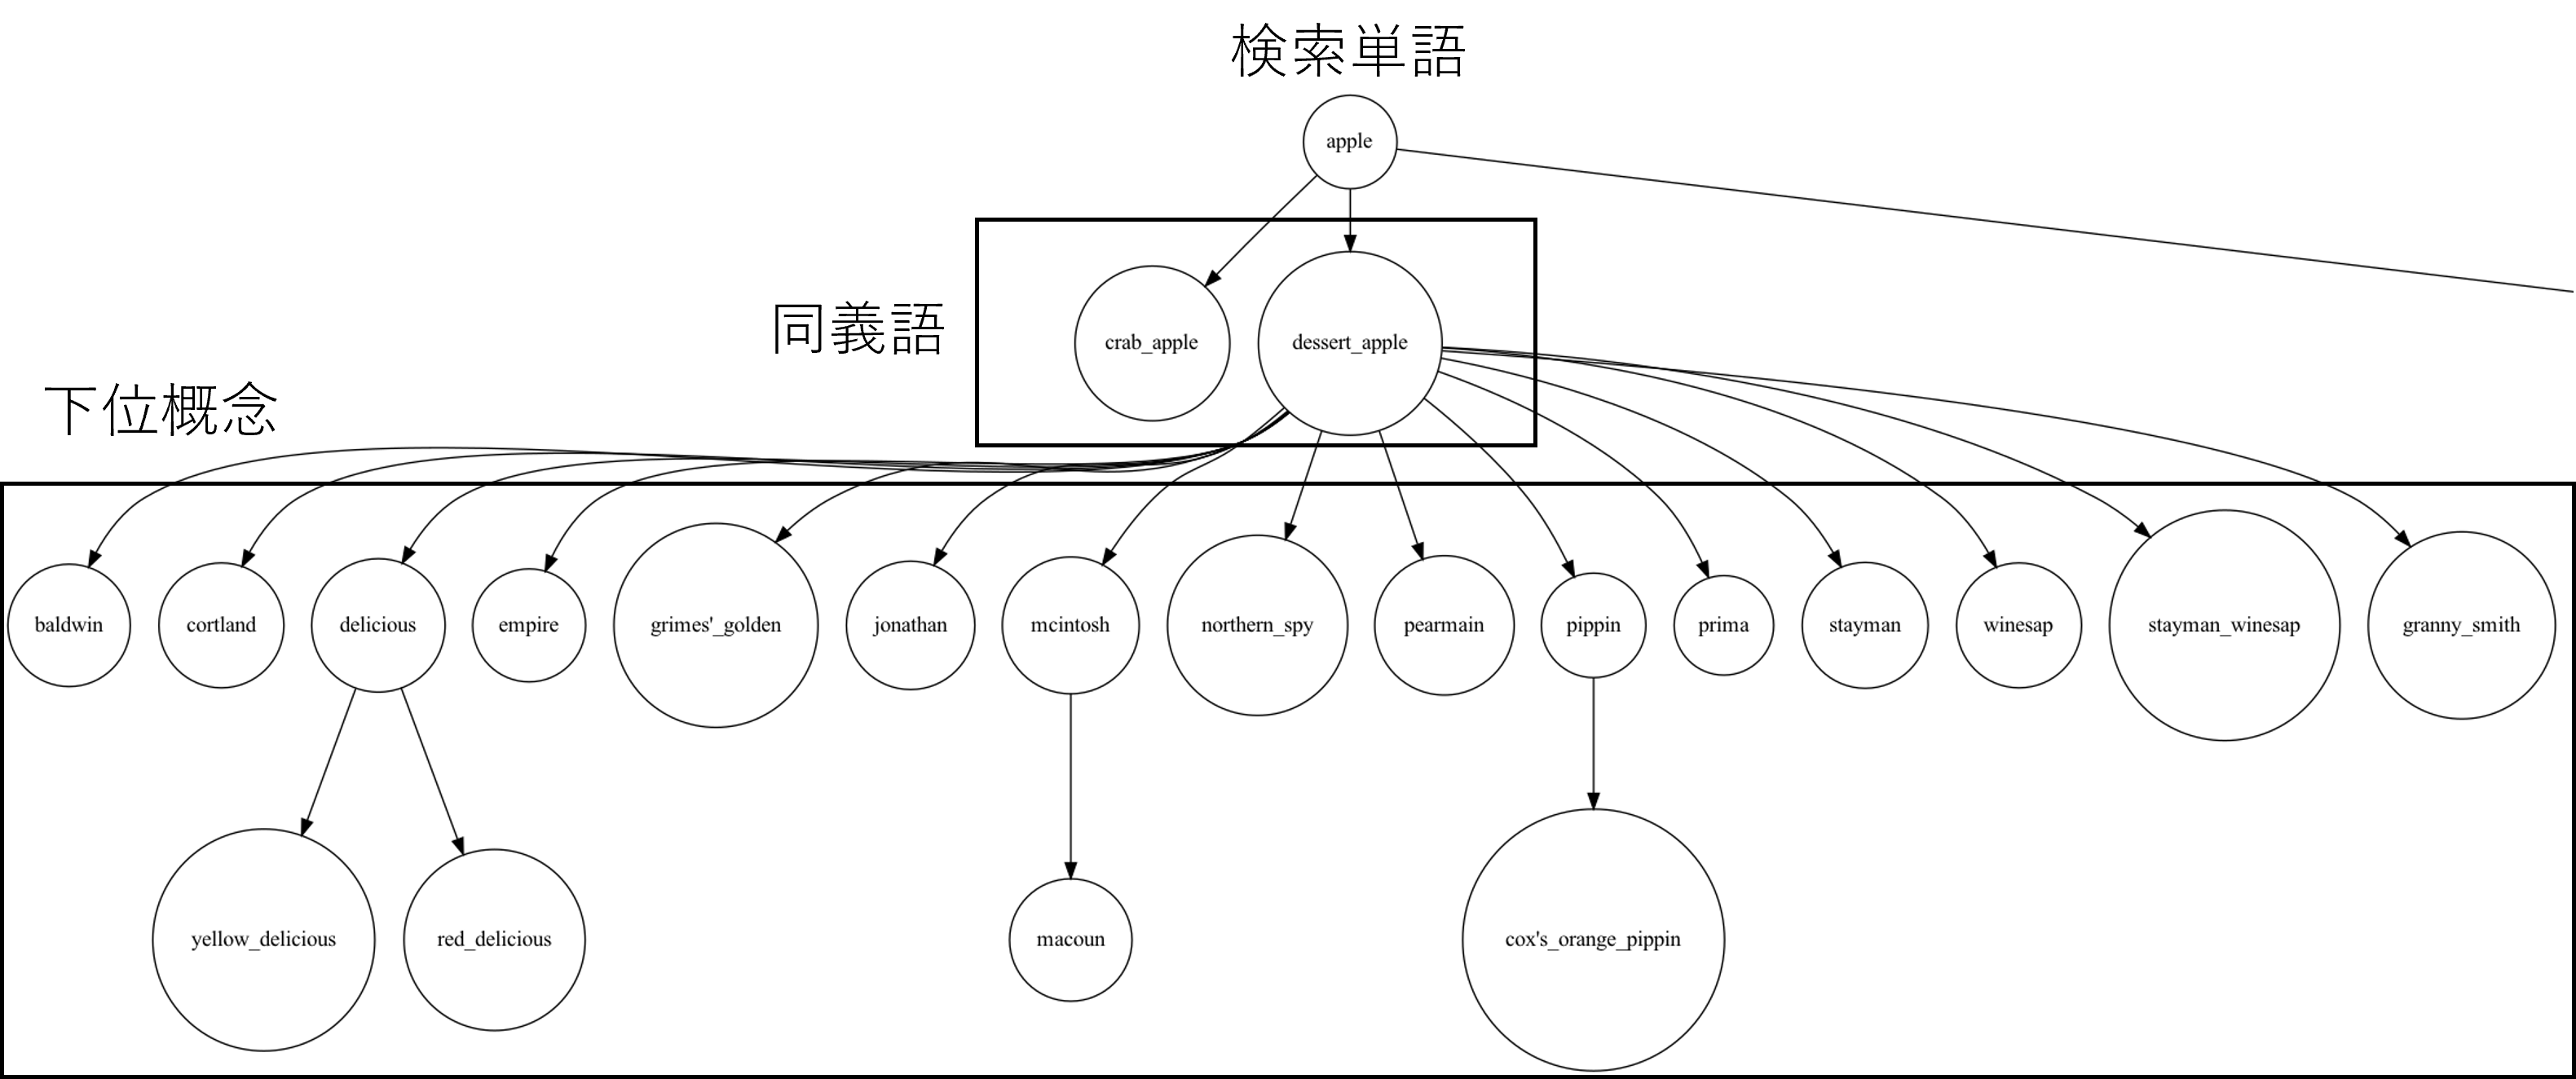
\includegraphics[width=1.0\columnwidth]{image/tree_structure.png}
        \caption{``りんご''を入力した際の下位概念の関係を表す木構造の例}
        \label{fig:tree_structure}
    \end{center}
\end{figure}

\section{Mecab}
\label{sec:mecab}
日本語の形態素解析を目的として、C++言語で開発されたオープンソースソフトウェアにMeCabがある\cite{mecab}。
MeCabを用いることによって、日本語で記述された文書の分かち書きや、単語の品詞を取得できる。

本研究では、自然言語仕様書から単語とその単語の品詞を取得するために、MeCabを用いて自然言語仕様書内の文を形態素解析する。

\section{TfidfVectorizer}
\label{sec:tfidf}
文書内の単語の特徴量を得る手法の1つとして、TF-IDF法(Term Frequency Inverse Document Frequency Method)
がある\cite{TF}。TF-IDF法は、特定の文書にだけ頻繁に現れる単語に、大きな重みを与えるTF法と、コーパス中の多数の文書に現れる単語に、あまり重みを与えないIDF法の、
2つの手法によって計算する手法である。この手法によって計算された値は、TF-IDF値と呼ばれる。
TF-IDFを計算するためのオープンソースライブラリの1つに、scikit-learnがある。
scikit-learnは、機械学習ライブラリを多様に用意しており、その中のTfidfVectorizerクラスを利用することで、TF-IDF値を計算できる\cite{cite6}。

本研究では、TfidfVectorizerを用いて、自然言語仕様書内の単語に対し、機械学習に必要なパラメータとしてTF-IDF値を計算する。

\section{ロジスティック回帰}
\label{sec:logistic}
ロジスティック回帰は、様々な種類の問題をモデル化することを目的として使用される統計手法の1つである。
統計学において、ある結果が起こる確率を予測する手段としてよく知られている手法であり、特に分類タスクで広く使われる。

式\ref{eq:logistic}に、ロジスティック回帰を示す。

\begin{equation}\label{eq:logistic}
    y = \log{(\frac{1}{1-p})}= \beta_{0}+ \beta_{1}\alpha_{1}+\beta_{2}\alpha_{2}+...+\beta_{x}\alpha_{x}
\end{equation}
$y$は、目的変数である確率$p$を説明変数$\alpha_{x}$と線形な関係になるように変換した値である。
$\beta_{0}$は、定数であり、$\beta_{1}~\beta_{x}$は、偏回帰変数である。

判定結果が2つのみの予測に使用できるロジスティック回帰を作成するために、2値ロジスティック回帰がある\cite{two_logistic}。
2値ロジスティック回帰は、$y$の値が0.5以上の場合は確率を1.0とみなし、0.5未満の場合は確率を0.0とみなすことによって、目的変数を判定する手法である。

式\ref{eq:two_logistic}に、2値ロジスティック回帰を示す。
式\ref{eq:logistic}をロジット変換で0から1に変換したものである。
\begin{equation}\label{eq:two_logistic}
    p = \frac{1}{1+exp[- (\beta_{0}+ \beta_{1}\alpha_{1}+\beta_{2}\alpha_{2}+...+\beta_{x}\alpha_{x})]}
\end{equation}

判定結果が3つ以上の予測に使用できるロジスティック回帰を作成するために、多項ロジスティック回帰がある\cite{multinomial_logistic}。
多項ロジスティック回帰は、目的変数がA、B、Cの3種類である場合、式\ref{eq:multi_logisticA}-式\ref{eq:multi_logisticC}の3つの式により、A、B、Cの確率をそれぞれ計算する。
さらに、最も大きい確率である目的変数を、判定結果とする。

\begin{equation}\label{eq:multi_logisticA}
    p_{A} = \frac{exp[(\beta_{10}+ \beta_{11}\alpha_{1}+\beta_{12}\alpha_{2}+...+\beta_{1x}\alpha_{x})]}{exp[(\beta_{20}+ \beta_{21}\alpha_{1}+\beta_{22}\alpha_{2}+...+\beta_{2x}\alpha_{x})]+exp[(\beta_{30}+ \beta_{31}\alpha_{1}+\beta_{32}\alpha_{2}+...+\beta_{3x}\alpha_{x})]}
\end{equation}

\begin{equation}\label{eq:multi_logisticB}
    p_{B} = \frac{exp[(\beta_{20}+ \beta_{21}\alpha_{1}+\beta_{22}\alpha_{2}+...+\beta_{2x}\alpha_{x})]}{exp[(\beta_{10}+ \beta_{11}\alpha_{1}+\beta_{12}\alpha_{2}+...+\beta_{1x}\alpha_{x})]+exp[(\beta_{30}+ \beta_{31}\alpha_{1}+\beta_{32}\alpha_{2}+...+\beta_{3x}\alpha_{x})]}
\end{equation}

\begin{equation}\label{eq:multi_logisticC}
    p_{C} = \frac{exp[(\beta_{30}+ \beta_{31}\alpha_{1}+\beta_{32}\alpha_{2}+...+\beta_{3x}\alpha_{x})]}{exp[(\beta_{10}+ \beta_{11}\alpha_{1}+\beta_{12}\alpha_{2}+...+\beta_{1x}\alpha_{x})]+exp[(\beta_{20}+ \beta_{21}\alpha_{1}+\beta_{22}\alpha_{2}+...+\beta_{2x}\alpha_{x})]}
\end{equation}

2値ロジスティック回帰と多項ロジスティック回帰のアルゴリズムを用いるモデルは「教師あり学習」手法である。
このため、モデルをトレーニングするための結果をあらかじめ含んだデータセットを用意する必要があり、
データをロジスティック関数にフィッティングすることで事象の発生確率を予測する。

既存ツールは、単語を、VDM++仕様書に必要である単語と、VDM++仕様書に必要でない単語の2つに分類するために、機械学習のモデルとして、2値ロジスティック回帰モデルを用いる。
VGMLは、単語を、VDM++仕様書に必要でない単語、VDM++仕様書に必要であるが、クラスの候補ではない単語、VDM++仕様書に必要であり、かつ、クラスの候補である単語の
3つに分類するために、機械学習のモデルとして、多項ロジスティック回帰モデルを用いる。